\chapter*{Revisión sistemática de la literatura}
\addcontentsline{toc}{chapter}{Revisión sistemática de la literatura}\label{cap:revisionLiteratura}

\section*{1. Construcción de la bitacóra}
\addcontentsline{toc}{section}{Construcción de la bitacóra}\label{cap:bitacora}
En búsqueda de una base teórica para la elección de una tecnología de virtualización basada en contenedores, 
se realizó una revisión del estado del arte. Esta revisión se completó en diferentes etapas: 

\subsection*{1.1 Planeación}
\addcontentsline{toc}{subsection}{Planeación}\label{cap:planeacion}
Esta etapa consistió en establecer el propósito general que se buscaba 
alcanzar con el SMS \textit{(Systematic mapping study)}.  A su vez, definió aspectos 
como objetivos, preguntas de investigación y métricas. Para ello, se siguió el 
modelo Objetivo-Pregunta-Métrica \textit{(GQM)} por su acrónimo en inglés. A continuación, 
se definen los objetivos del SMS aplicado a las tecnologías de virtualización basadas en contenedores.

\subsubsection{1.1.1 Definición de metas para el SMS}
\addcontentsline{toc}{subsubsection}{Definición de metas para el SMS}\label{cap:metasSMS}

\begin{table}[H]
    \centering
    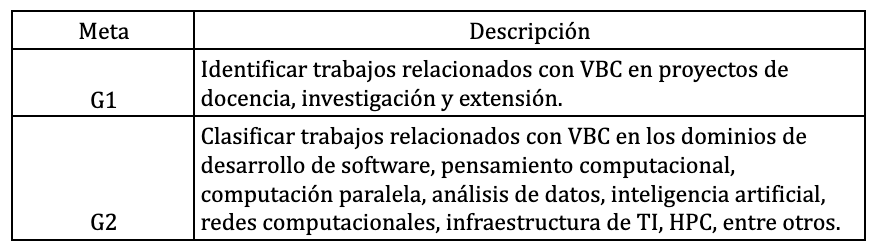
\includegraphics[width=\textwidth] {tablas-images/cp2/definicionMetas.png}
    \caption{Definición de metas del SMS}\label{tab:tabla-metas}
\end{table}

\subsubsection{1.1.2 Definición de preguntas de investigación}
\addcontentsline{toc}{subsubsection}{Definición de preguntas de investigación}\label{cap:preguntasInvestigacion}

\begin{table}[H]
    \centering
    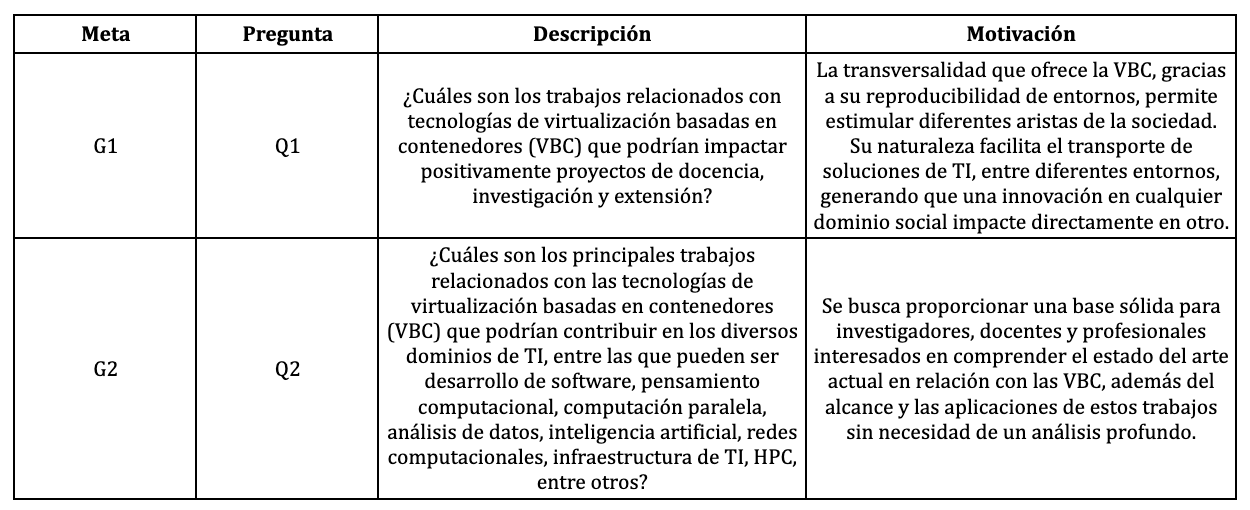
\includegraphics[width=\textwidth] {tablas-images/cp2/preguntasInvestigacion.png}
    \caption{Definición de preguntas de investigación del SMS}\label{tab:tabla-preguntas}
\end{table}

\subsubsection{1.1.3 Definición de métricas}
\addcontentsline{toc}{subsubsection}{Definición de métricas}\label{cap:metricasSMS}

\begin{figure}[H]
    \centering
    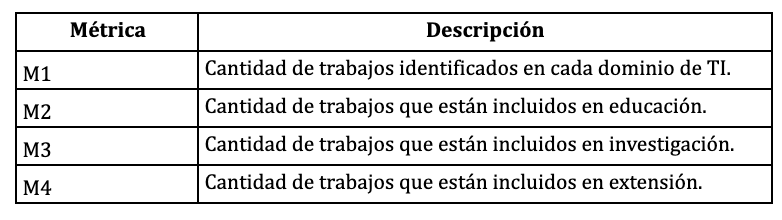
\includegraphics[width=\textwidth] {tablas-images/cp2/definicionMetricas.png}
    \caption{Definición de métricas del SMS}\label{fig:tabla-metricas}
\end{figure}

\section*{2. Búsqueda de estudios}
\addcontentsline{toc}{section}{Búsqueda de estudios}\label{cap:busquedaEstudios}
Esta etapa comprendió las siguientes secciones: 
1) Estrategia de búsqueda, ya sea independiente o combinada; 
2) Identificación general de estudios; 
3) Selección y, finalmente, 
4) Selección de estudios para incluir en el SMS.